
\begin{frame}[t]{Modelos de simulación de la ecología del vector.}
  \begin{center}
   \begin{columns}[T]
        \begin{column}[T]{4cm}
             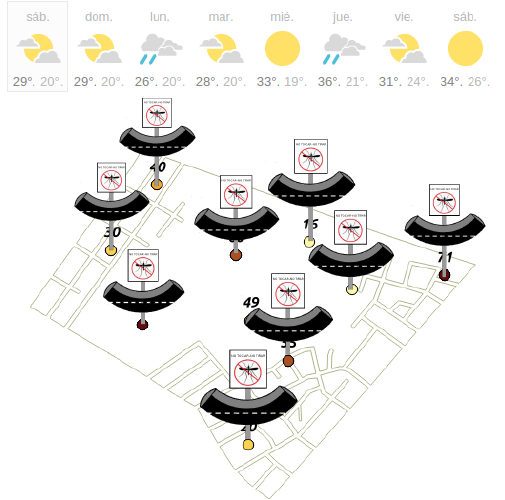
\includegraphics[width=4.5cm]{./graphics/larvitrmpas-clima.png}
        \end{column}
        \begin{column}[T]{7cm}
          \begin{itemize}
          \item Larvitrampas como puntos de control.
          \item Conteo de larvas mediante PDI.
          \item Influencia de las variaciones climáticas.
          \item Combinar información regionalizada, meteorológica y geográfica.
          \item Simular el comportamiento del vector.
          \item Detección temprana de posibles focos y en consecuencia una posible epidemia.
          \end{itemize}
        \end{column}
    \end{columns}
  \end{center}
\end{frame}

\begin{frame}[t]{Modelos de simulación de la ecología del vector.\\\textit{Modelo matemático del ciclo de vida.}}
  \begin{center}
   \begin{columns}[t]
        \begin{column}[T]{7cm}
            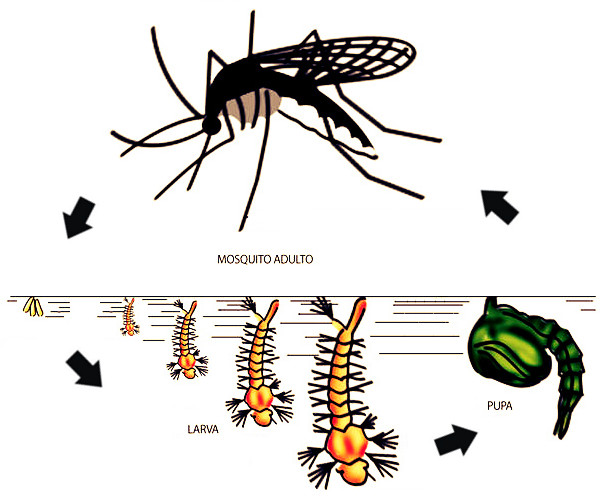
\includegraphics[width=7cm]{./graphics/ciclo-de-vida.jpg}
        \end{column}
        \begin{column}[T]{4cm}
          \begin{itemize}
            \item Tasas de desarrollo.
            \item Tasas de mortalidad.
            \item Dispersión.
            \item Ciclo gonotrófico.
            \item Ovipostura.
          \end{itemize}
        \end{column}
    \end{columns}
  \end{center}
\end{frame}

\begin{frame}[c]{Modelos de simulación de la ecología del vector.\\\textit{Modelo matemático del ciclo de vida.}}
  \begin{center}
   \begin{columns}[T]
        \begin{column}[T]{6cm}
            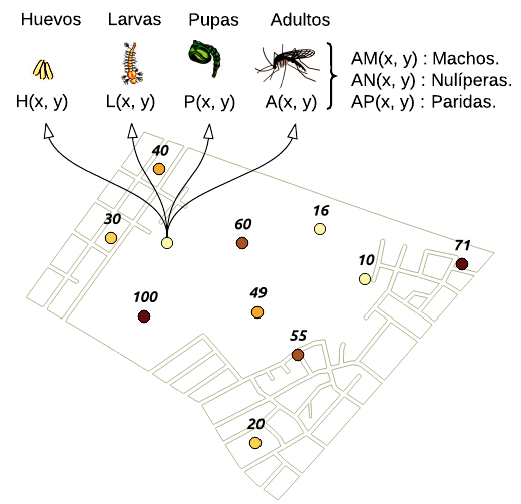
\includegraphics[width=6cm]{./graphics/modelado-poblacion.png}
        \end{column}
        \begin{column}[T]{5.5cm}
          \begin{itemize}
            \item $H(x, y)$ : Huevos.
            \item $L(x, y)$ : Larvas.
            \item $P(x, y)$ : Pupas.
            \item $AM(x, y)$ : Adultos machos.
            \item $AN(x, y)$ : Hembras nulíperas.
            \item $AP(x, y)$ : Hembras paridas.
          \end{itemize}
        \end{column}
    \end{columns}
  \end{center}
\end{frame}


\begin{frame}[c]{Modelos de simulación de la ecología del vector.\\\textit{Zonificación.}}

  \begin{center}
   \begin{columns}[T]
        \begin{column}[T]{4cm}
              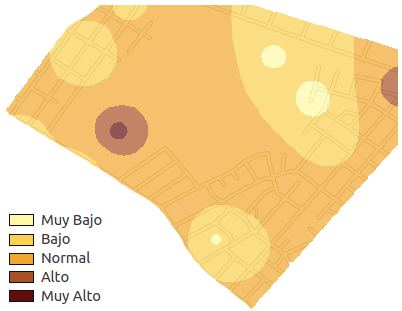
\includegraphics[width=\textwidth]{./graphics/zonificacion-intro.png}
        \end{column}
        \begin{column}[T]{6cm}
          \textit{\\Cada entorno puede contar con factores que lo hagan más o menos apta para el desarrollo, mortalidad, alimentación, dispersión y reproducción de individuos.}
        \end{column}
    \end{columns}
  \end{center}
\end{frame}

\begin{frame}[c]{Modelos de simulación de la ecología del vector.\\\textit{Zonificación.}}
  \begin{center}
   \begin{columns}[T]
        \begin{column}[T]{5cm}
            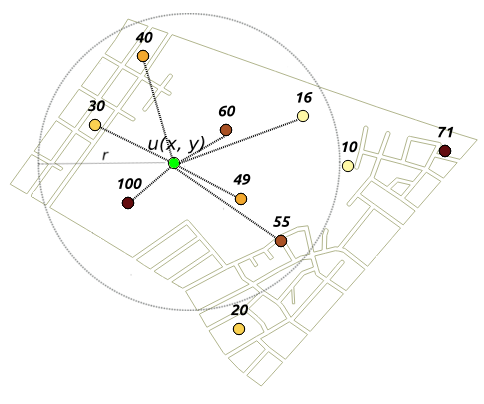
\includegraphics[width=5.5cm]{./graphics/zonificacion.png}
        \end{column}
        \begin{column}[T]{6cm}
          \begin{itemize}
          \item Los puntos de control permiten caracterizar la zona como más o menos apta para el desarrollo, mortalidad, alimentación, dispersión y reproducción.
          \item Interpolación espacial para determinar la cantidad de individuos en $(x, y)$.
          \item Definir una escala de clasificación.
          \end{itemize}
        \end{column}
    \end{columns}
  \end{center}
\end{frame}


\begin{frame}[t]{Modelos de simulación de la ecología del vector.\\\textit{Zonificación (Interpolación Espacial).}}
  \begin{center}
   \begin{columns}[T]
        \begin{column}[T]{3.5cm}
            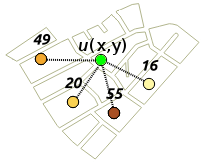
\includegraphics[width=4cm]{./graphics/interpolacion-ej.png}
        \end{column}
        \begin{column}[T]{7cm}
        \begin{equation}\label{eq:interpolacion-idw}
         u(X) = \sum_{i=1}^{N} w_i(X) * u_{i}
        \end{equation}
        Donde :
        \begin{equation}
        w_i(X) =  \dfrac{d(X, X_i)^{-p}}{\sum_{j=1}^{N} d(X, X_i)^{-p}}
        \end{equation}
        \end{column}
    \end{columns}
  \end{center}
    \text{Ejemplo:}
    $u(x,y) = w_1(x,y) * 49 + w_2(x,y) * 20 + w_3(x,y) * 55 + w_4(x,y) * 16 $
\end{frame}



\begin{frame}[c]{Modelos de simulación de la ecología del vector.\\\textit{Zonificación.}}
  Consideraciones para la clasificación de las zonas:
  \begin{itemize}
      \item El $50$ \% de las larvas observadas son hembras.
      \item La temperatura media anual es de 25 \textcelsius.
      \item La tasa mortalidad diaria natural de las larvas y pupas bajo optimas condiciones, a 25 \textcelsius, es igual a $0,01056\ \text{días}^{-1}$ respectivamente.
      \item El desarrollo, a 25 \textcelsius, de la larva hasta su emergencia a adulto es de $11,57$ días.
      \item El $32,10$ \% de las hembras adultas no oviponen.
  \end{itemize}
\end{frame}

\begin{frame}[t]{Modelos de simulación de la ecología del vector.\\\textit{Zonificación.}}

  \begin{table}
        \begin{minipage}{\textwidth}
          \centering
          \scriptsize
            \caption{\label{tab:cap4-puntaje-zona} Escala de clasificación de las zonas
            para el desarrollo, alimentación, dispersión y reproducción.}
            \begin{tabular}{l c c c c}
                \hline
                             & Mínimo$^a$ & Máximo$^a$ & Hembras$^b$ & Hembras$^c$ \\
                Tipo de zona & $u(x,y)$   & $u(x,y)$   & Adultas     & Reproductivas \\
                \hline
                \hline
                Pésima  & 0  & 19 & 8  & 5 \\
                Mala    & 20 & 35 & 15 & 10\\
                Regular & 36 & 51 & 22 & 15\\
                Buena   & 52 & 69 & 30 & 20\\
                Óptima  & 70 & --$^d$ & --$^d$ & --$^d$
            \end{tabular}
            \footnotetext[1]{\scriptsize Rango mínimo y máximo de $u(x,y)$ permitido para el tipo de zona.}
            \footnotetext[2]{\scriptsize Cantidad máxima de hembras adultas, al final del periodo de desarrollo.}
            \footnotetext[3]{\scriptsize Cantidad de hembras adultas con capacidad de oviponer.}
            \footnotetext[4]{\scriptsize No se estableció un límite superior para las zonas óptimas. }
        \end{minipage}
    \end{table}
\end{frame}

%Tasas de desarrollo.
\begin{frame}[c]{Modelos de simulación de la ecología del vector.\\\textit{Tasas de desarrollo.}}
  \begin{center}
   \begin{columns}[T]
        \begin{column}[T]{6.5cm}
            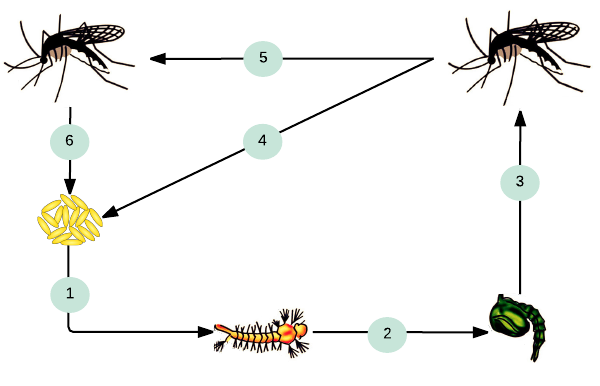
\includegraphics[width=7cm]{./graphics/tasas-desarrollo.png}
        \end{column}
        \begin{column}[T]{5cm}
          \begin{enumerate}
            \item Eclosión de huevos.
            \item Emergencia de pupas.
            \item Emergencia de adultos.
            \item Ciclo gonotrófico para hembras nulíperas.
            \item Ciclo gonotrófico para hembras paridas.
          \end{enumerate}
        \end{column}
    \end{columns}
  \end{center}
\end{frame}

\begin{frame}[t]{Modelos de simulación de la ecología del vector.\\\textit{Tasas de desarrollo
 (Sharpe y DeMichele, 1977).}}
  \begin{center}
      \begin{equation} \label{eq:schoolfield}
         R(k)  = R(298K) *\cfrac{ \cfrac{k}{298K} *
          exp \Bigg[
                  \cfrac{\Delta H_{A}}{R} \bigg(\cfrac{1}{298K} - \cfrac{1}{k}\bigg)
              \Bigg]}
          {1 + exp\Bigg[\cfrac{\Delta H_{H}}{R} \bigg(\cfrac{1}{T_{1/2}}- \cfrac{1}{k}\bigg)\Bigg] }
      \end{equation}
  \end{center}
   \begin{itemize}
      \item $R(k)$ : Tasa de desarrollo media ($dias^{-1}$).
      \item $\Delta H_{A}$ y $\Delta H_{H}$ : son entalpías termodinámicas características del organismo.
      \item $T_{1/2}$ es la temperatura cuando la mitad de la enzima se desactiva.
      \item $R$ : es la constante universal de los gases.
      \item $k$ : Temperatura en Kelvin.
    \end{itemize}
\end{frame}


\begin{frame}[c]{Modelos de simulación de la ecología del vector.\\\textit{Tasas de Mortalidad.}}
  \begin{itemize}
      \item Simular la reducción de la población por la mortalidad.
      \item La mortalidad depende de la etapa del ciclo de desarrollo.
      \item Las poblaciones cuentan con una cantidad entera de individuos.
      \item Determinar la cantidad de individuos que deben ser eliminados de la población.
      \item La cantidad de individuos a eliminar debe ser entera.
  \end{itemize}
\end{frame}

\begin{frame}[c]{Modelos de simulación de la ecología del vector.\\\textit{Mortalidad de los huevos(Otero et al., 2006).}}
  % poseen una gran resistencia
  \begin{center}
      \begin{equation}
          M_{H(x,y)} = me * H(x,y)
      \end{equation}
  \end{center}
  Donde :
    \begin{itemize}
      \item $me$ : Tasa de mortalidad diaria igual a $0,01\  \text{días}^{-1}$.
      \item $H(x, y)$ : Cantidad de huevos observados en $(x,y)$.
      \item $M_{H(x,y)}$ : Cantidad de huevos a eliminar.
    \end{itemize}
\end{frame}

\begin{frame}[c]{Simulación del proceso evolutivo. \\\textit{Mortalidad bajo óptimas condiciones.}}
  Mortalidad bajo óptimas condiciones de las larvas y pupas (Otero et al., 2006) :
  \begin{center}
    \begin{equation}
    \label{eq:mortalidad-natural-larvas}
        mo(k) = 0.01 + 0.9725 * exp\bigg( \frac{-(k - 278)}{2.7035}\bigg)
    \end{equation}
  \end{center}
  Donde :
    \begin{itemize}
      \item $k$ : Temperatura en Kelvin.
    \end{itemize}
\end{frame}

\begin{frame}[c]{Modelos de simulación de la ecología del vector.\\\textit{Mortalidad de larvas (Otero et al., 2006).}}
  \begin{center}
      \begin{equation}
      M_{L(x,y)}(k) = mo(k) * L(x,y) + \bigg(\frac{\alpha _{0}}{BS(x,y)}\bigg) * L(x,y) *(L(x,y) - 1)
    \end{equation}
  \end{center}
  Donde:
 \begin{itemize}
      \item $k$ : Temperatura en Kelvin.
      \item $L(x, y)$ : Cantidad de larvas observadas en $(x,y)$.
      \item $\alpha _{0}$ : Capacidad de carga de un solo lugar de reproducción.
      \item $BS(x,y)$ : Es el número de sitios de reproducción en $(x,y)$ .
      \item $M_{L(x,y)}$ : Cantidad de larvas a eliminar.
    \end{itemize}
\end{frame}

\begin{frame}[c]{Modelos de simulación de la ecología del vector.\\\textit{Mortalidad de las pupas (Otero et al., 2006).}}
  \begin{center}
    \begin{equation}
        M_{P(x,y)}(k) = P(x,y) * (mo(k) + (1 - ef) * R(k))
    \end{equation}
  \end{center}
  Donde :
    \begin{itemize}
      \item $k$ : Temperatura en Kelvin.
      \item $ef$ : el factor de supervivencia es de $0,83$.
      \item $P(x, y)$ : Cantidad de pupas observadas en $(x,y)$.
      \item $M_{P(x,y)}$ : Cantidad de pupas a eliminar.
    \end{itemize}
\end{frame}

\begin{frame}[c]{Modelos de simulación de la ecología del vector.\\\textit{Mortalidad de adultos (Otero et al., 2006).}}
 % 10% diario, 50% semanal, 95% a final del primer mes.
  % Es constante, a pesar de su alta mortalidad, si la población
  % es lo sifucientemente grande, puede llegar a causar una epidemia
  \begin{center}
    \begin{equation}
        M_{A(x,y)} = ma * A(x,y)
    \end{equation}
  \end{center}
  Donde:
    \begin{itemize}
      \item $ma$ : Tasa de mortalidad diaria igual a $0,09$ \ $1/\text{días}$.
      \item $A(x, y)$ : Cantidad de adultos observados en $(x,y)$.
      \item $M_{A(x,y)}$ : Cantidad de adultos a eliminar.
    \end{itemize}
\end{frame}


\begin{frame}[c]{Modelos de simulación de la ecología del vector.\\\textit{Ciclo gonotrófico y Ovipostura.}}
  \begin{center}
      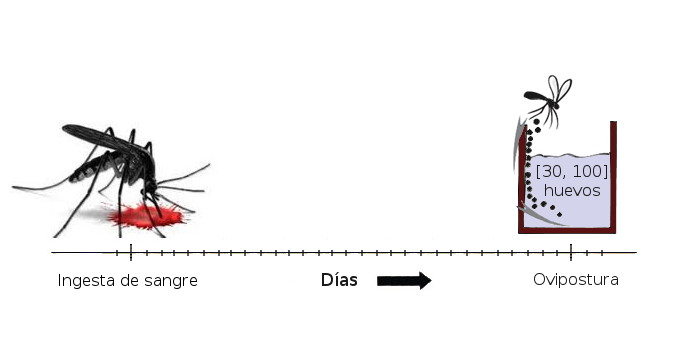
\includegraphics[width=9.5cm]{./graphics/cliclo-gonotrofico-tiempo.jpg}
  \end{center}
\end{frame}

\begin{frame}[t]{Modelos de simulación de la ecología del vector.\\\textit{Dispersión.}}
  \begin{center}
    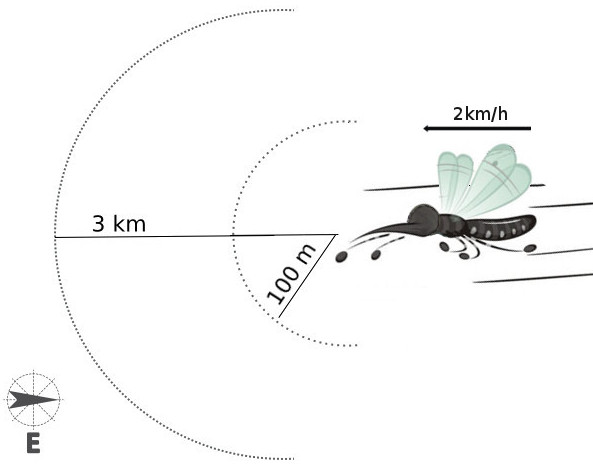
\includegraphics[width=7.5cm]{./graphics/dispersion.jpg}
  \end{center}
\end{frame}

\begin{frame}[c]{Simulación del proceso evolutivo}
  \begin{center}
    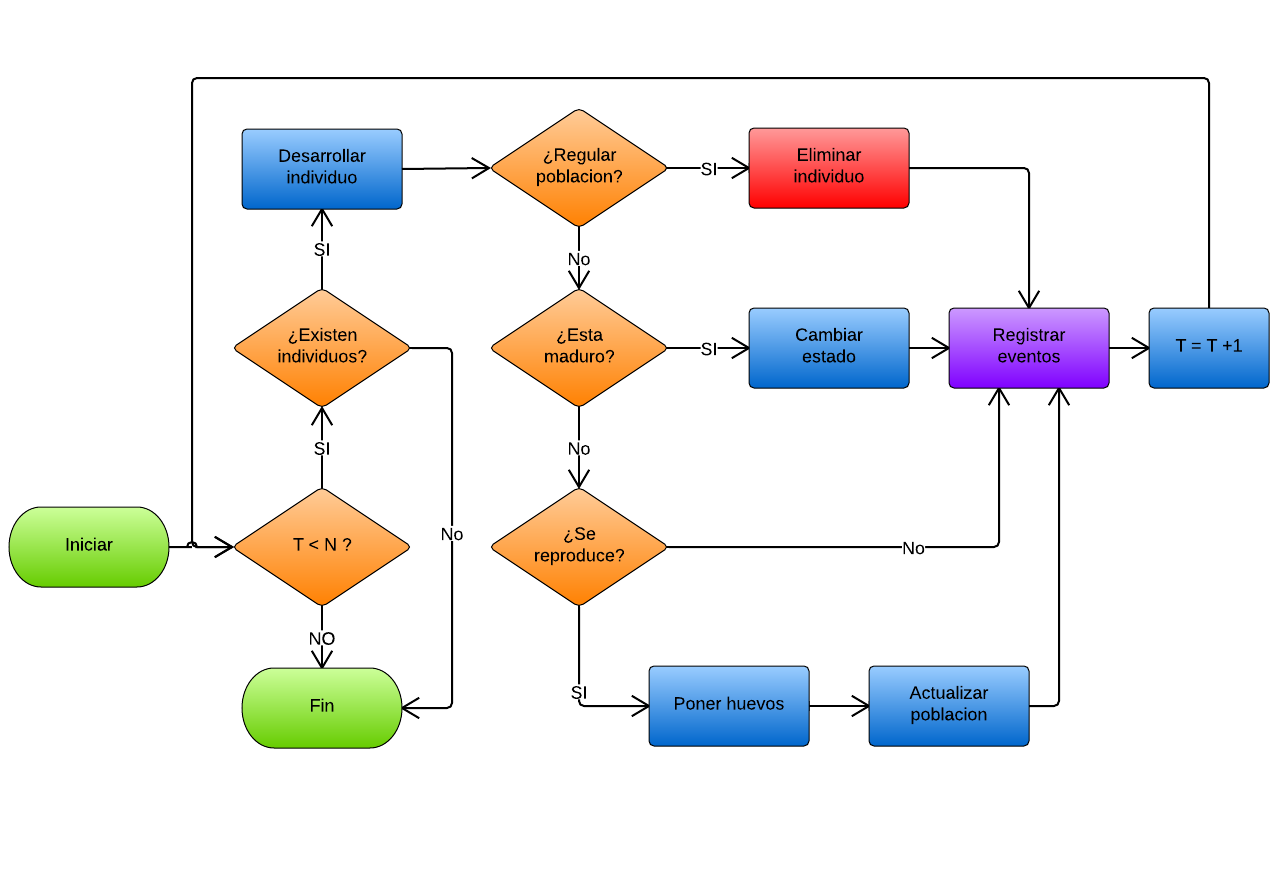
\includegraphics[height=7.5cm]{./graphics/algoritmo-propuesto.png}
  \end{center}
\end{frame}

